\chapter{IUGONETメタデータ作成・登録}

\section{メタデータ作成・登録の流れ}
図\ref{flow.eps}の手順で、メタデータの作成・登録を進めます。
\begin{figure}[H]
\begin{center}
\fbox{
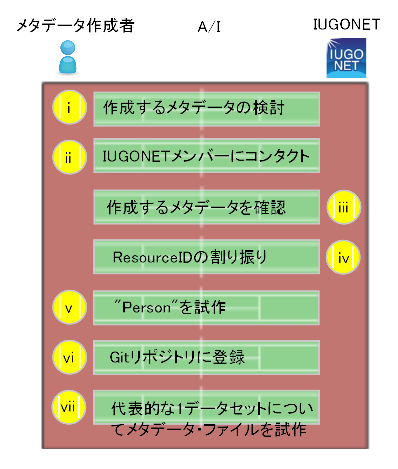
\includegraphics[width=12cm]{images/flow.eps}
}
\caption{メタデータ作成・登録のワークフロー}
\label{flow.eps}
\end{center}
\end{figure}

\renewcommand{\thesubsection}{(\roman{subsection})}
\subsection{作成するメタデータの検討}\label{check}

まず初めに、作成するメタデータを検討し、表\ref{initial}を埋めて下さい。(現時点で埋めれるだけで、
結構です。)

\begin{table}[H]
\begin{center}
\caption{作成するメタデータに関する質問表}
\label{initial}
\begin{tabular}{ll|l}\hline
1. & 登録データセットの名前 & \ \ \ \ \ \ \ \ \ \ \ \ \ \ \ \ \ \ \ \ \ \ \ \ \ \ \ \ \ \ \ \ \ \ \ \ \ \ \ \ \ \ \ \ \ \ \ \ \ \ \ \ \ \\
2. & データセットに関する簡単な説明 & \\
3. & Principal Investigatorの名前 & \\
4. & Principal Investigatorの所属 & \\
5. & メタデータ作成者の名前 & \\
6. & メタデータ作成者の所属 & \\
7. & データセットのアクセスポリシー & (公開、制限付き公開、非公開など) \\ \hline
\end{tabular}
\end{center}
\end{table}

\subsection{IUGONETメンバーにコンタクト}\label{contact}
表\ref{initial}の内容を添付し、表\ref{contact}のIUGONET開発メンバーにEmailを送付して下さい。

\begin{table}[H]
\begin{center}
\caption{IUGONETメタデータに関する連絡先一覧。特に希望がない場合は、IUGONET大代表に連絡して下さい。(専門分野が近い者が、IUGONET側の担当になります。)}
\label{contact}
\begin{tabular}{lllll}\hline
機関 & 担当者 & Email& & ([at]は@と読み替えて下さい。)\\ \hline
\cellcolor[gray]{0.9}IUGONET大代表 & \cellcolor[gray]{0.9}- & \cellcolor[gray]{0.9}iugonet2009 & \cellcolor[gray]{0.9}[at] & \cellcolor[gray]{0.9}gmail.com\\ 
東北大・理・PPARC & 八木 学 & yagi & [at] & pparc.tohoku.ac.jp\\
極地研 & 田中 良昌 & ytanaka & [at] & nipr.ac.jp\\
  & 佐藤 由佳 & sato.yuka & [at] & nipr.ac.jp\\
名大・STE研 & 堀 智昭 & horit & [at] & stelab.nagoya-u.ac.jp\\
京大・理・附属地磁気センター & 小山 幸伸 & ykoyama & [at] & kugi.kyoto-u.ac.jp\\
京大・理・附属天文台 & 上野 悟 & ueno & [at] & kwasan.kyoto-u.ac.jp\\
京大・生存圏研究所 & 谷田貝 亜紀代 & akiyo\_yatagai & [at] & rish.kyoto-u.ac.jp\\
 & 新堀 淳樹 & shinbori & [at] & rish.kyoto-u.ac.jp\\
九大・ICSWSE & 阿部 修司 & abeshu & [at] & serc.kyushu-u.ac.jp\\ \hline
\end{tabular}
\end{center}
\end{table}

\subsection{作成するメタデータセットの確認}
IUGONET共通メタデータ・フォーマット\footnote{http://www.iugonet.org/mdformat.html}に則って、メタデータをXML形式\footnote{Extensible Markup Language, http://www.w3.org/TR/REC-xml/}で記述します。
データセットに関するメタデータ以外に、観測装置、観測サイト、に関する
メタデータ等を別々のXMLファイルに作成し、相互にリンクします(図\ref{flow.eps})。
後述するResourceIDを指し示すことで、この相互リンクを確立します。

\begin{figure}[H]
\begin{center}
\fbox{
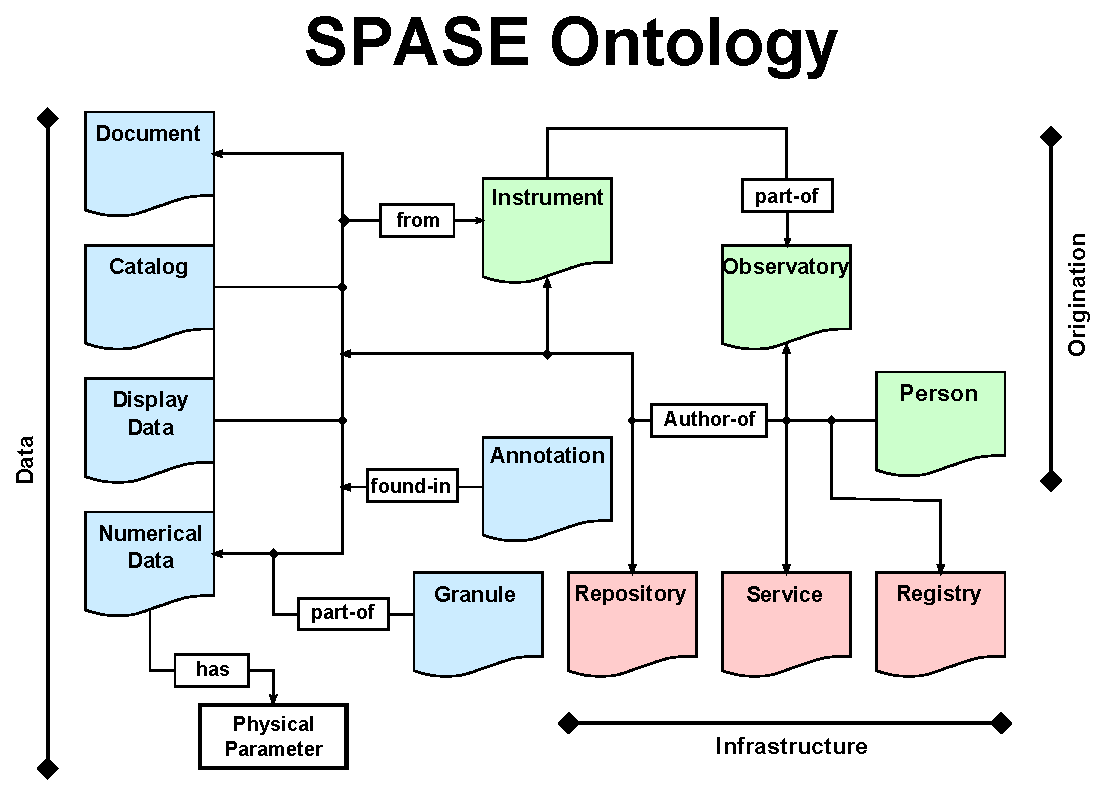
\includegraphics[width=12cm]{images/spaseOntology.eps}
}
\caption{SPASE Ontologyのダイアグラム。図中のNumericalDataが、いわゆるデータセットに関するメタデータに該当します。}
\label{spaseOntology}
\end{center}
\end{figure}

\begin{table}[H]
\begin{center}
\caption{リソース・タイプの説明}
\begin{tabular}{ll}\hline
Annotation & Information which is explanatory or descriptive which is associated \\
 & with another resource.\\
Catalog & A tabular listing of events or observational notes, especially those \\
 & that have utility in aiding a user in locating data. Catalogues include lists of events, \\
 & files in a product, and data availability. A Catalog resource is a type of "data product" \\
 & which is a set of data that is uniformly processed and formatted, from one or more \\
 & instruments, typically spanning the full duration of the observations of the relevant \\ 
 & instrument(s). A data product may consist of a collection of granules of successive \\
 & time spans, but may be a single high-level entity.\\
DisplayData & A graphical representation of data wherein the underlying numeric values \\
 & are not (readily) accessible for analysis. Examples are line plots and spectrograms. \\
 & A Display Data resource is a type of "data product" which is a set of data that is \\ 
 & uniformly processed and formatted, from one or more instruments, typically spanning the \\
 & full duration of the observations of the relevant instrument(s). A data product may \\
 & consist of a collection of granules of successive time spans, but may be a single \\ 
 & high-level entity.\\
Document & A set of information designed and presented as an individual entity. A document \\
 & may contain plain or formatted text, in-line graphics, sound, other multimedia data, or \\
 & hypermedia references. A Document resource is intended for use on digital objects that \\
 & have no other identifier (e.g., DOI or ISBN).\\
Granule  & An accessible portion of another resource. A Granule may be composed of one or \\
 & more physical pieces (files) which are considered inseparable. For example, a data storage \\
 & format that maintains metadata and binary data in separate, but tightly coupled files. \\
 & Granules should not be used to group files that have simple relationships or which are \\
 & associated through a parent resource. For example, each file containing a time interval \\
 & data for a Numerical Data resource would each be considered a Granule. The ParentID of a \\
 & Granule resource must be a NumericalData resource. The attributes of a Granule supersede \\
 & the corresponding attributes in the NumericalData resource.\\
Instrument & A device that makes measurements used to characterize a physical phenomenon, or \\
 & a family of like devices.\\
NumericalData & Data stored as numerical values in a specified format. A Numerical Data resource \\
 & is a type of "data product" which is a set of data that is uniformly processed and formatted, \\
 & from one or more instruments, typically spanning the full duration of the observations of the \\
 & relevant instrument(s). A data product may consist of a collection of granules of successive \\
 & time spans, but may be a single high-level entity.\\ \hline
Observatory & The host (spacecraft, network, facility) for instruments making observations, or a \\
 & family of closely related hosts.\\
Person & An individual human being. \\ \hline
Repository & A location or facility where resources are stored.\\
Registry & A location or facility where resources are cataloged.\\ 
Service & A location or facility that can perform a well defined task.\\ \hline
\end{tabular}
\end{center}
\end{table}


\begin{figure}[H]
\begin{center}
\fbox{
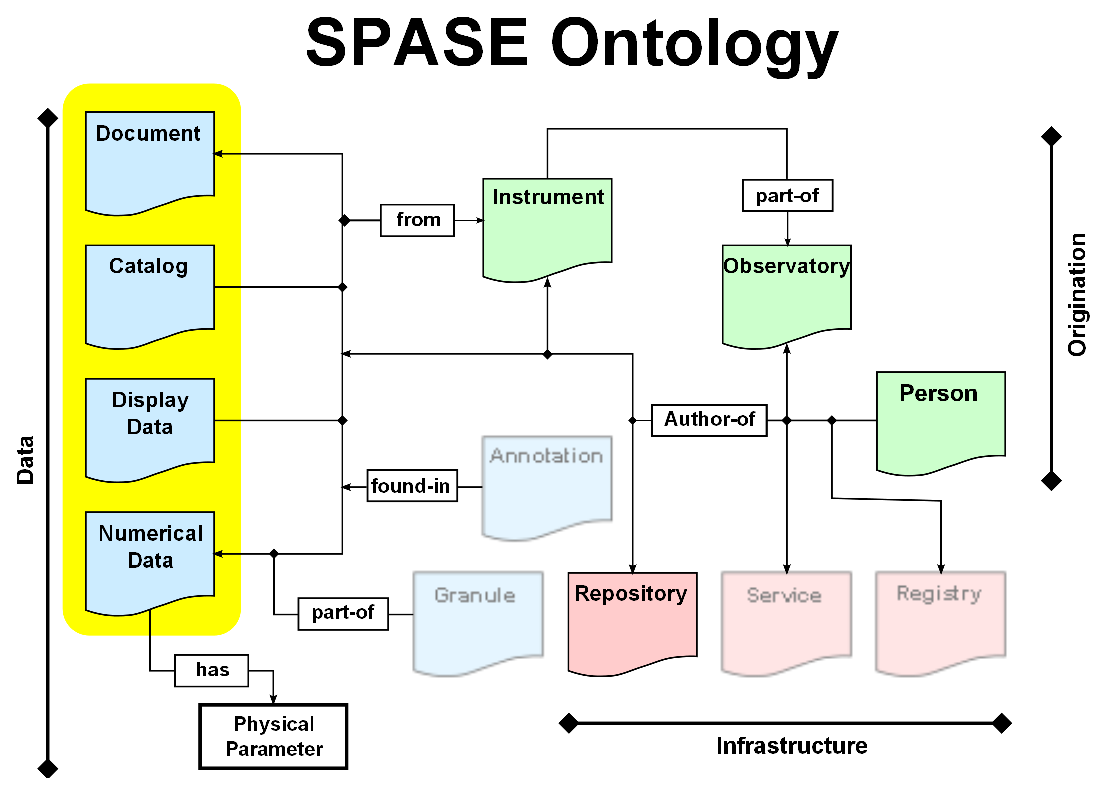
\includegraphics[width=12cm]{images/spaseOntology2.eps}
}
\caption{最小限のメタデータ種。黄色い枠内のいずれか1種+その他の4つのメタデータ種、が最小限のメタデータです。}
\label{spaseOntology2}
\end{center}
\end{figure}

メタデータを作成する場合、
\begin{itemize}
\item データセットのメタデータ
\item 観測機器のメタデータ
\item 観測サイトのメタデータ
\item PI, metadata contactなど人的リソースのメタデータ(Person\index{Person@Person})
\item データベースのメタデータ(Repository\index{Repository@Repository})
\end{itemize}
のように、最低5つのメタデータを作成することになります。括弧の中は、それぞれのメタデータ種の名前です。\par
 また観測データのデータファイル毎の検索を行えるようにするためには、以下のカテゴリーのメタデータを作成する
必要があります。\par
\begin{itemize}
\item 個々のデータファイルのメタデータ(Granule\index{Granule@Granule})
\end{itemize}
これは1つのデータファイルにつき1つ作成するので、非常に大量(データファイルの数と同じ)になります。\par
 メタデータの作成責任者の方と、IUGONETメンバーの担当者とで相談・確認した上で、最終的に幾つのデータセットの
メタデータを作成するか、またそれに付随して観測機器、観測サイト、人的リソース、データベースをそれぞれ幾つ
作成するかを決めます。対話的に。

\subsection{ResourceIDの割り振り}
 次に、各メタデータに付加されるユニークなIDを割り当てます。IUGONET共通メタデータ
フォーマットでは、このIDをResourceIDと呼びます。ResourceIDは、
\begin{screen}
\begin{verbatim}
spase://IUGONET/NumericalData/WDC_Kyoto/WDC/AE/index/PT1M_quicklook
\end{verbatim}
\end{screen}
の様なURI形式\footnote{Uniform Resource Identifier, http://tools.ietf.org/html/rfc3986}で表され、
\begin{screen}
\begin{verbatim}
spase://IUGONET/メタデータ種/研究機関コード/データグループ/データ名/.../...
\end{verbatim}
\end{screen}
のような構造になっています。メタデータ種は、図\ref{spaseOntology}の12種のメタデータ種から選択します。
ResourceIDは、他のメタデータ固有のResourceIDと重複してはいけない為、IUGONETメンバーと相談の上で決定
されます。

\subsection{Gitリポジトリに登録}

作成したメタデータの内容を精査した上で、間違いがなければそれをGitリポジトリに登録します。
登録には2つの方法があります。1つは、IUGONETメンバーの担当者にEmailで送付して、代理登録
してもらう方法です。メタデータの個数が少ない場合はこの方法で十分でしょう。2つめは、
IUGONETのメタデータの受付サーバーに自分で直接登録する方法です。
これには、gitというバージョン管理ソフトウェアの知識が必要となります。これに関しては、
◎◎を参照してください。









